\subsubsection{Biểu đồ số phép so sánh}


\paragraph{1. Dữ liệu ngẫu nhiên}
\begin{figure}[H]
    \centering
    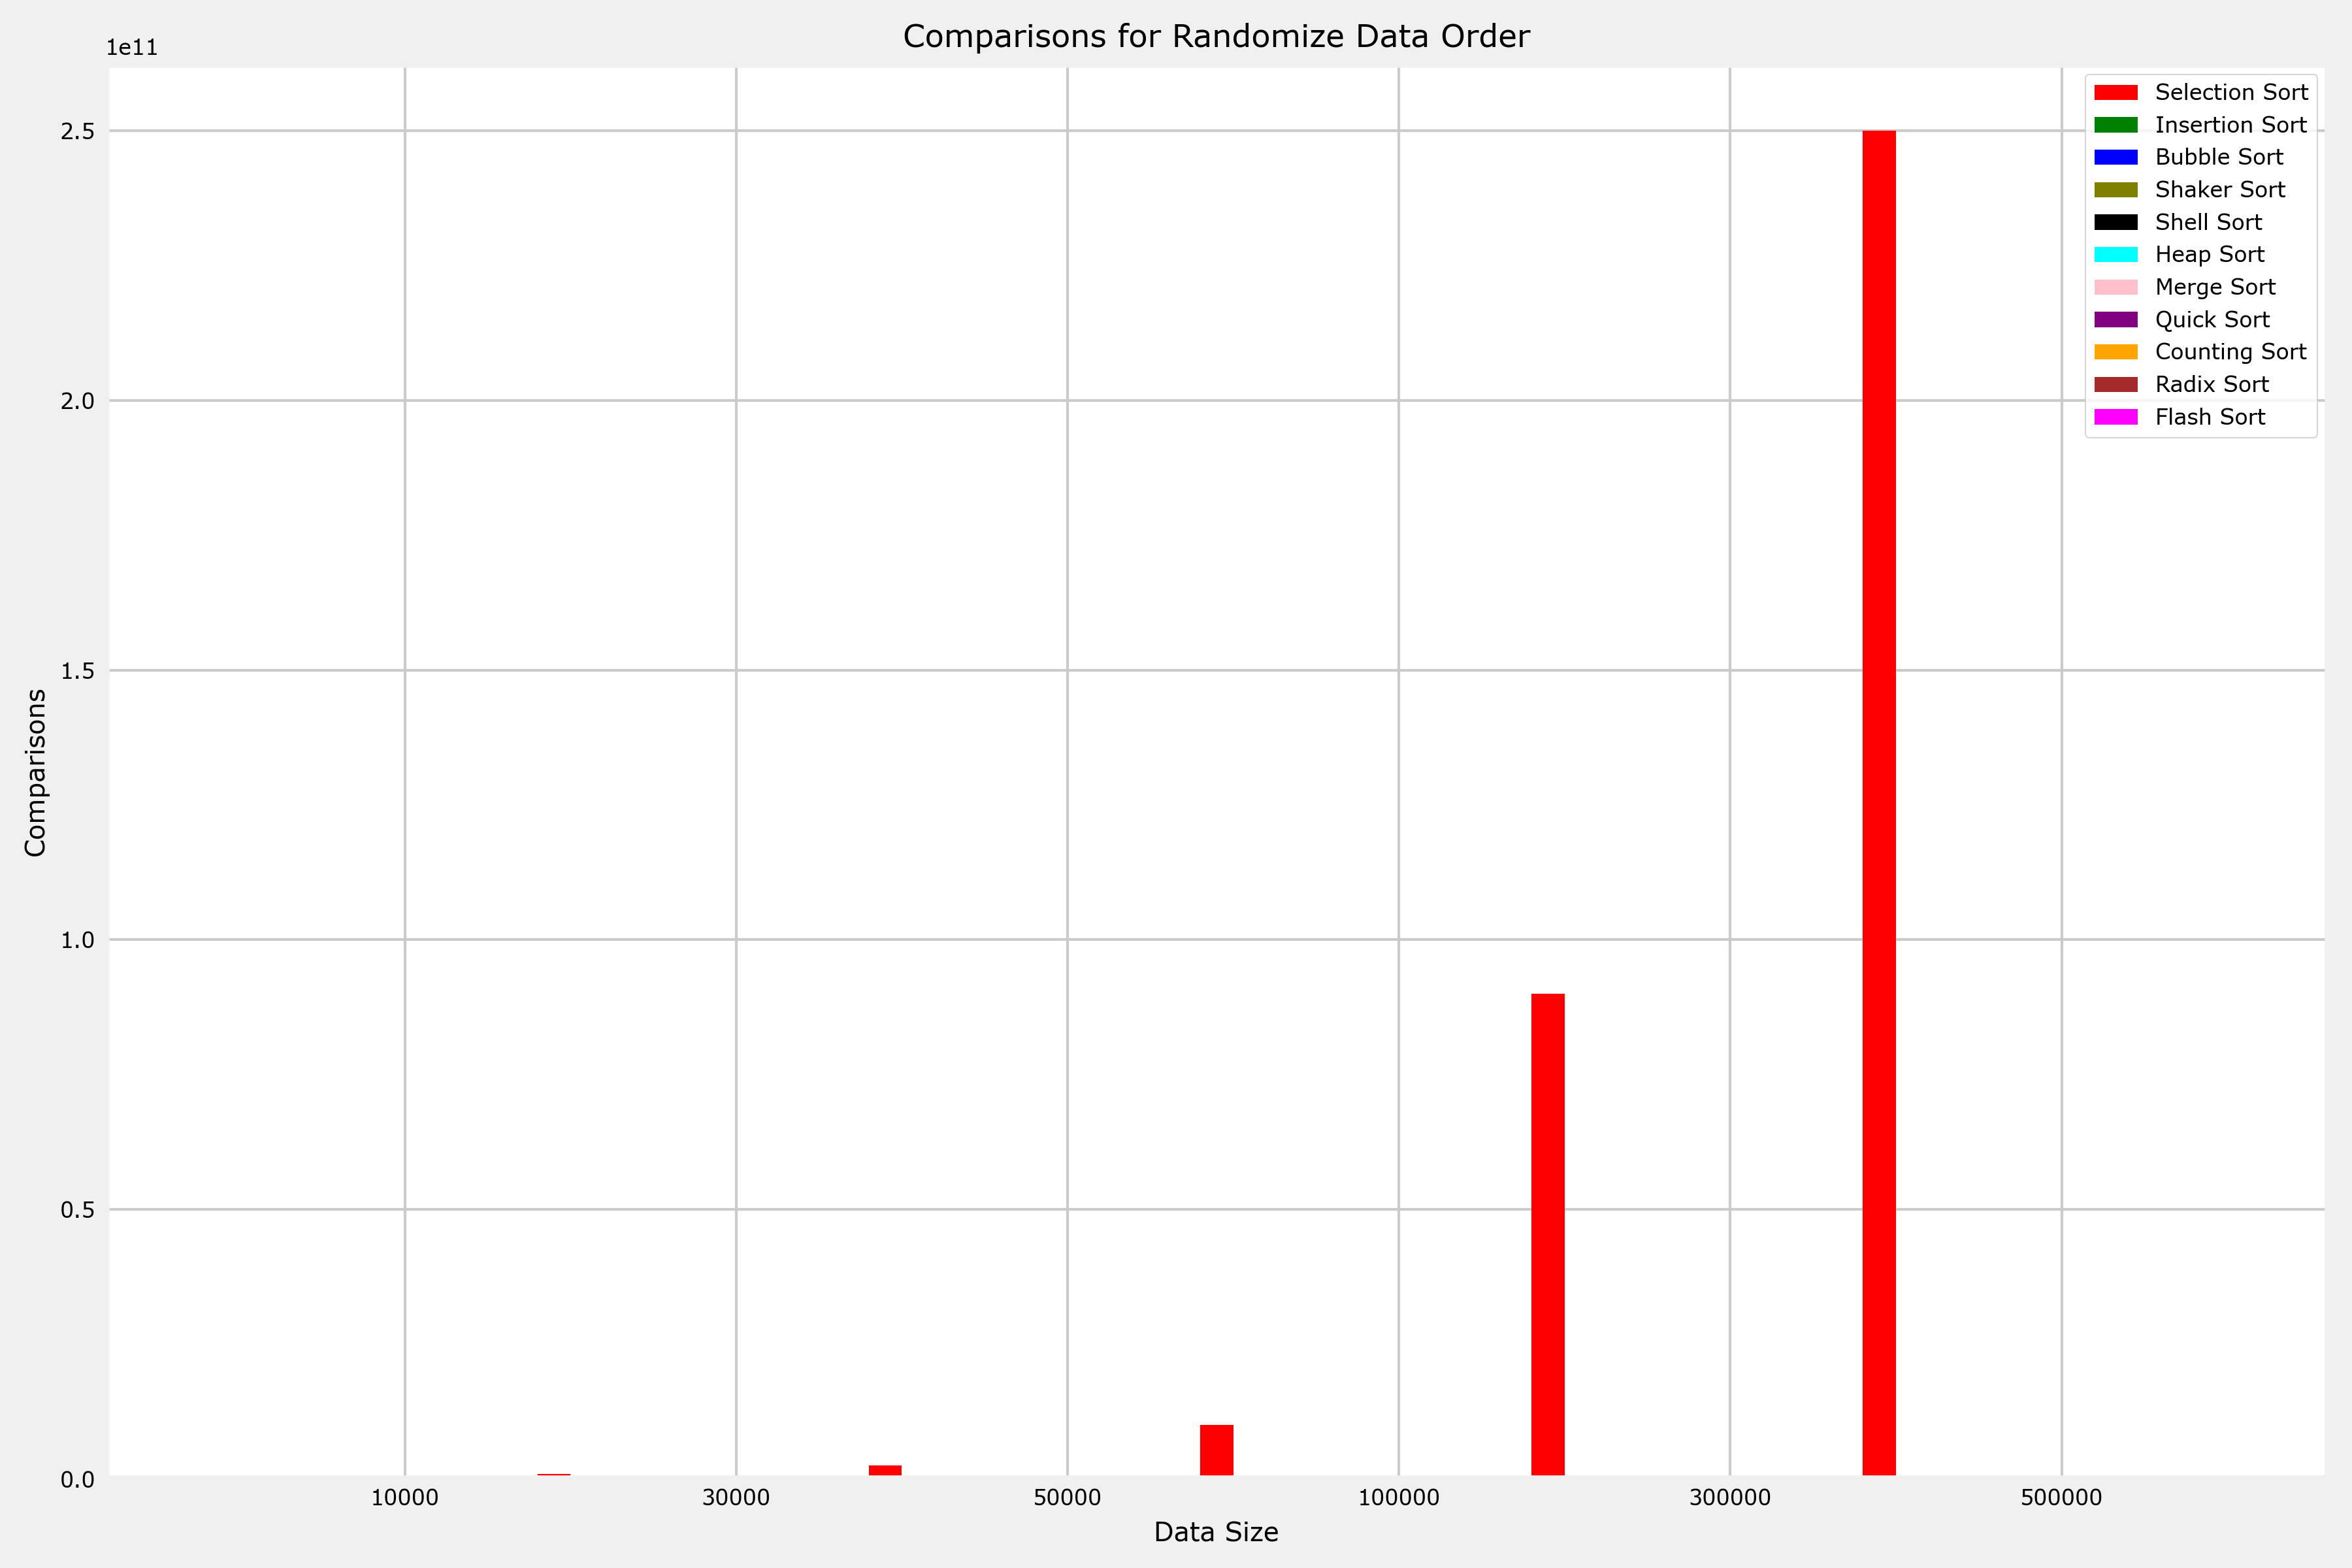
\includegraphics[width=0.8\textwidth]{img/results/randomize_comparisons.png}
    \caption{Số phép so sánh của 11 thuật toán với dữ liệu ngẫu nhiên}
\end{figure}

\begin{figure}[H]
    \centering
    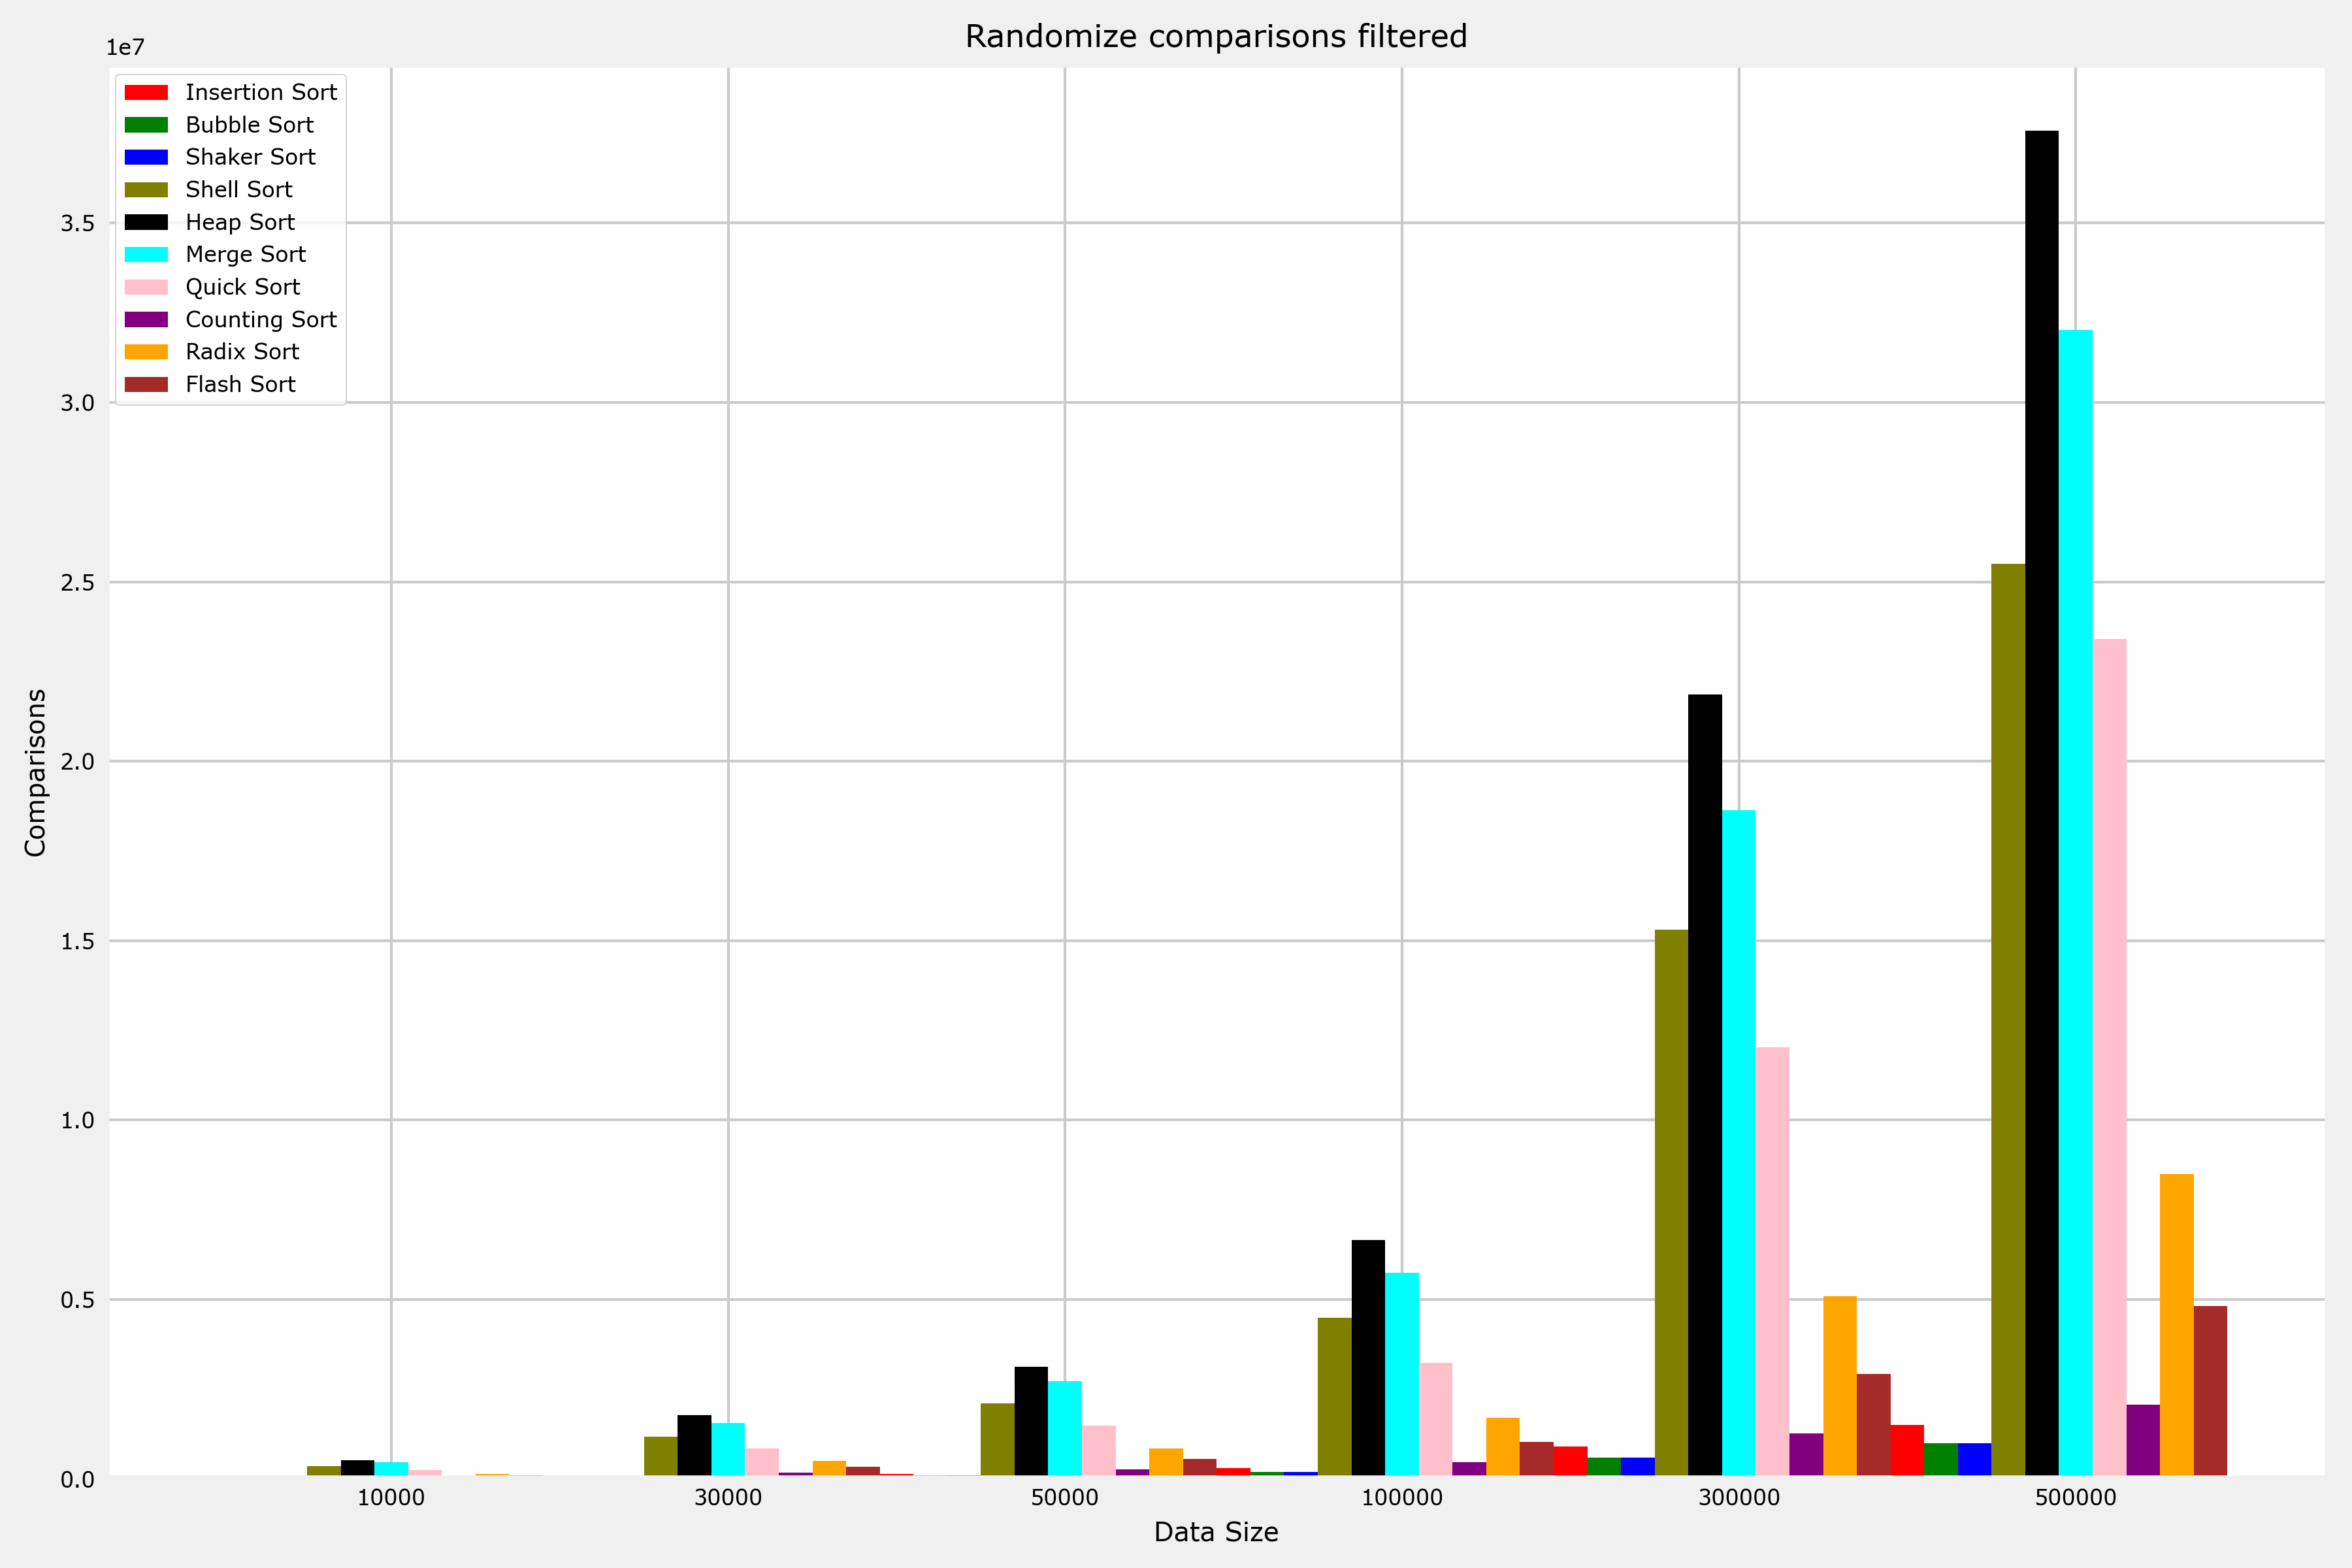
\includegraphics[width=0.8\textwidth]{img/results/randomize_comparisons_filtered.png}
    \caption{Số phép so sánh của 11 thuật toán với dữ liệu ngẫu nhiên sau khi loại bỏ outlier}
\end{figure}



\paragraph{2. Dữ liệu gần sắp xếp hoàn chỉnh}
\begin{figure}[H]
    \centering
    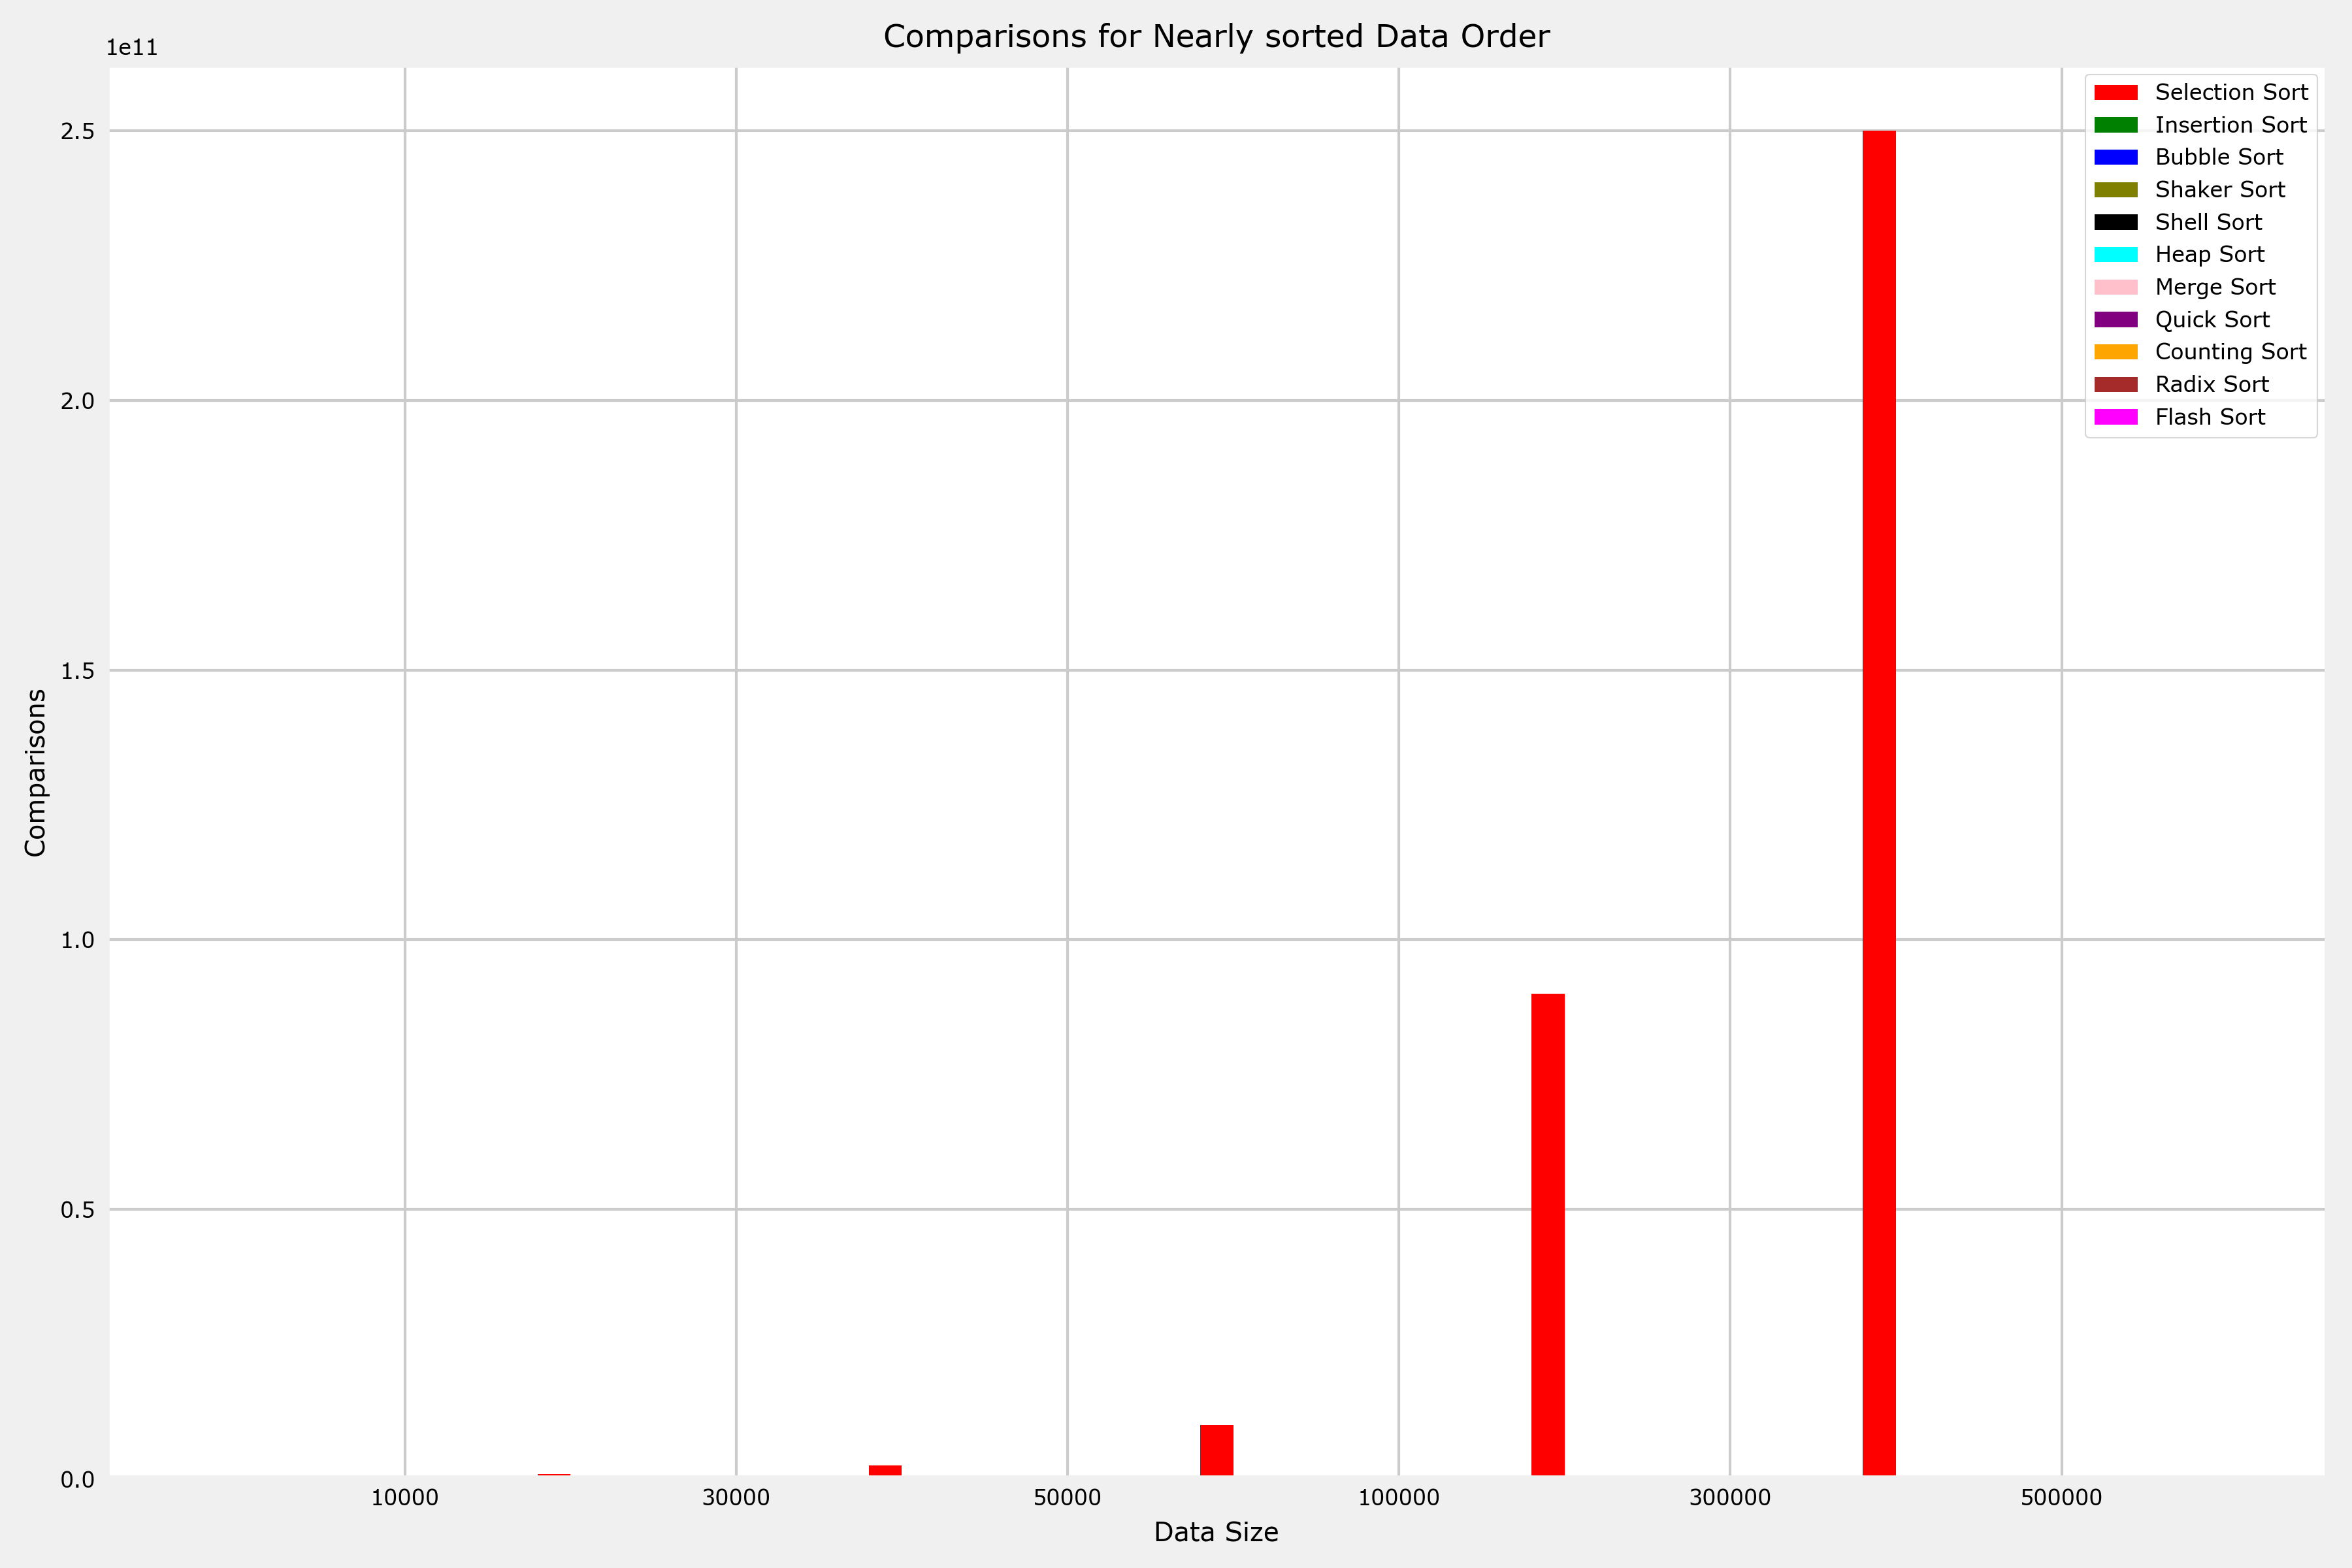
\includegraphics[width=0.8\textwidth]{img/results/nearly_sorted_comparisons.png}
    \caption{Số phép so sánh của 11 thuật toán với dữ liệu gần sắp xếp hoàn chỉnh}
\end{figure}

\begin{figure}[H]
    \centering
    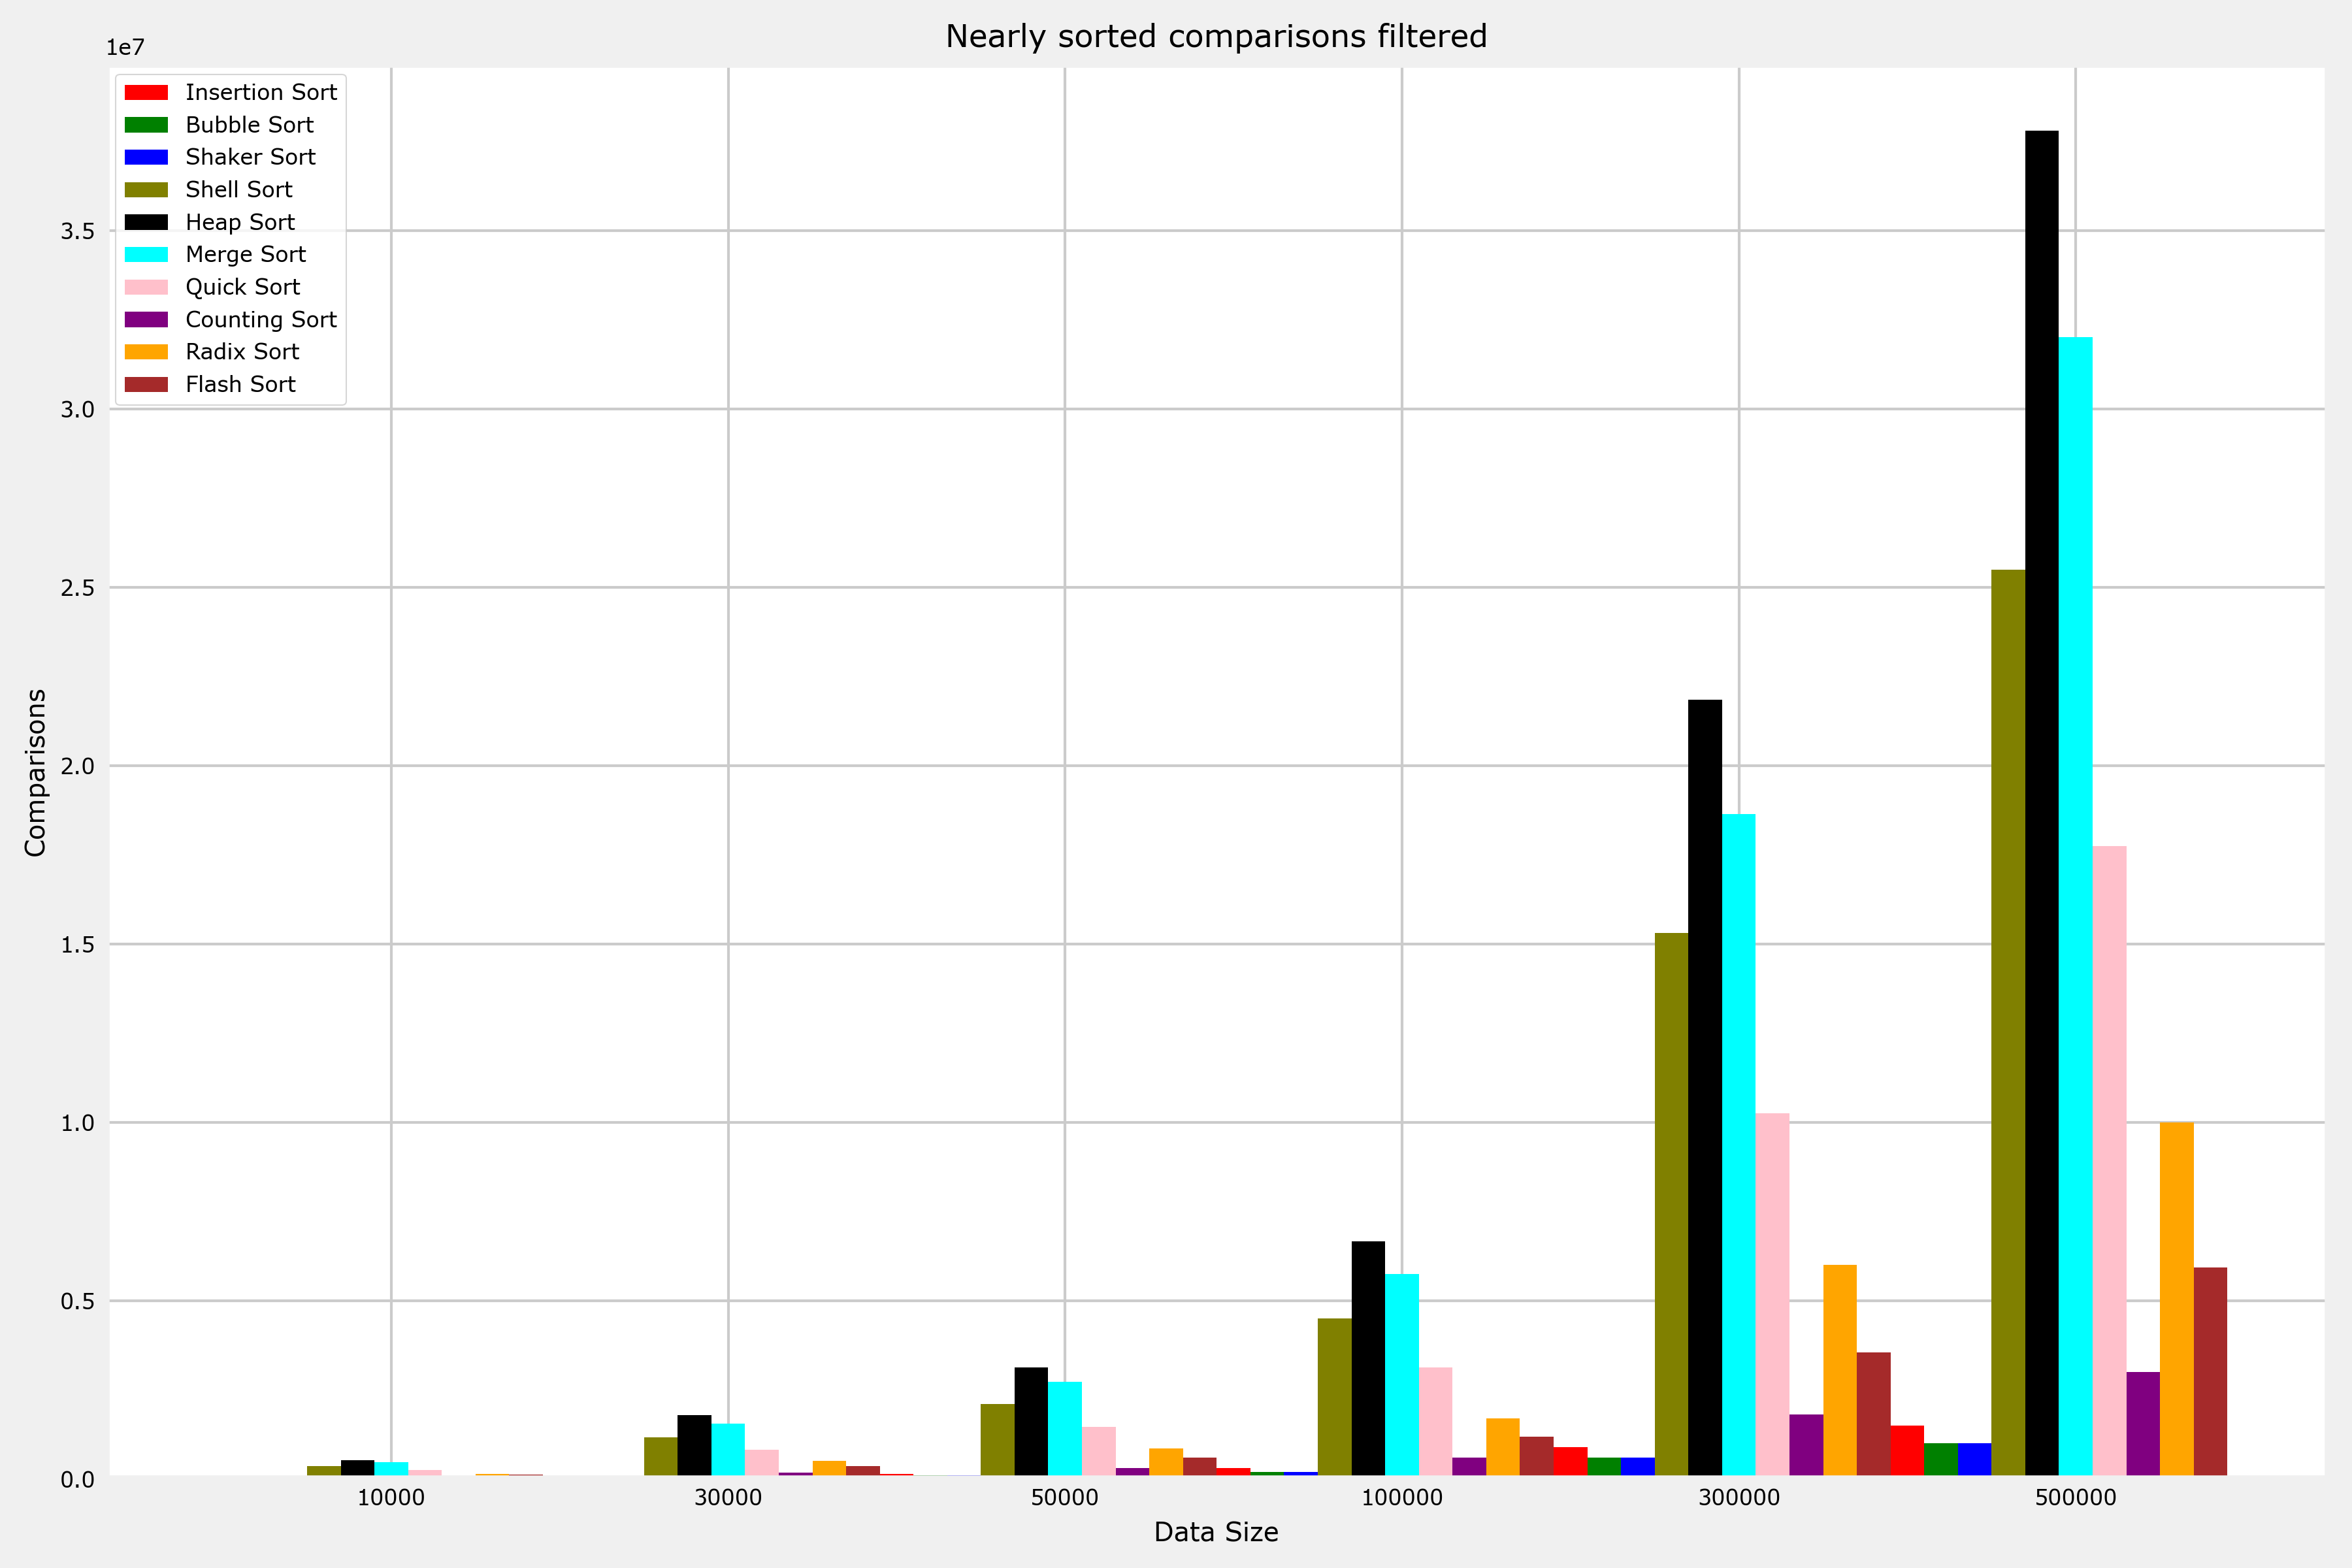
\includegraphics[width=0.8\textwidth]{img/results/nearly_sorted_comparisons_filtered.png}
    \caption{Số phép so sánh của 11 thuật toán với dữ liệu gần sắp xếp hoàn chỉnh sau khi loại bỏ outlier}
\end{figure}


\paragraph{3. Dữ liệu được sắp xếp}
\begin{figure}[H]
    \centering
    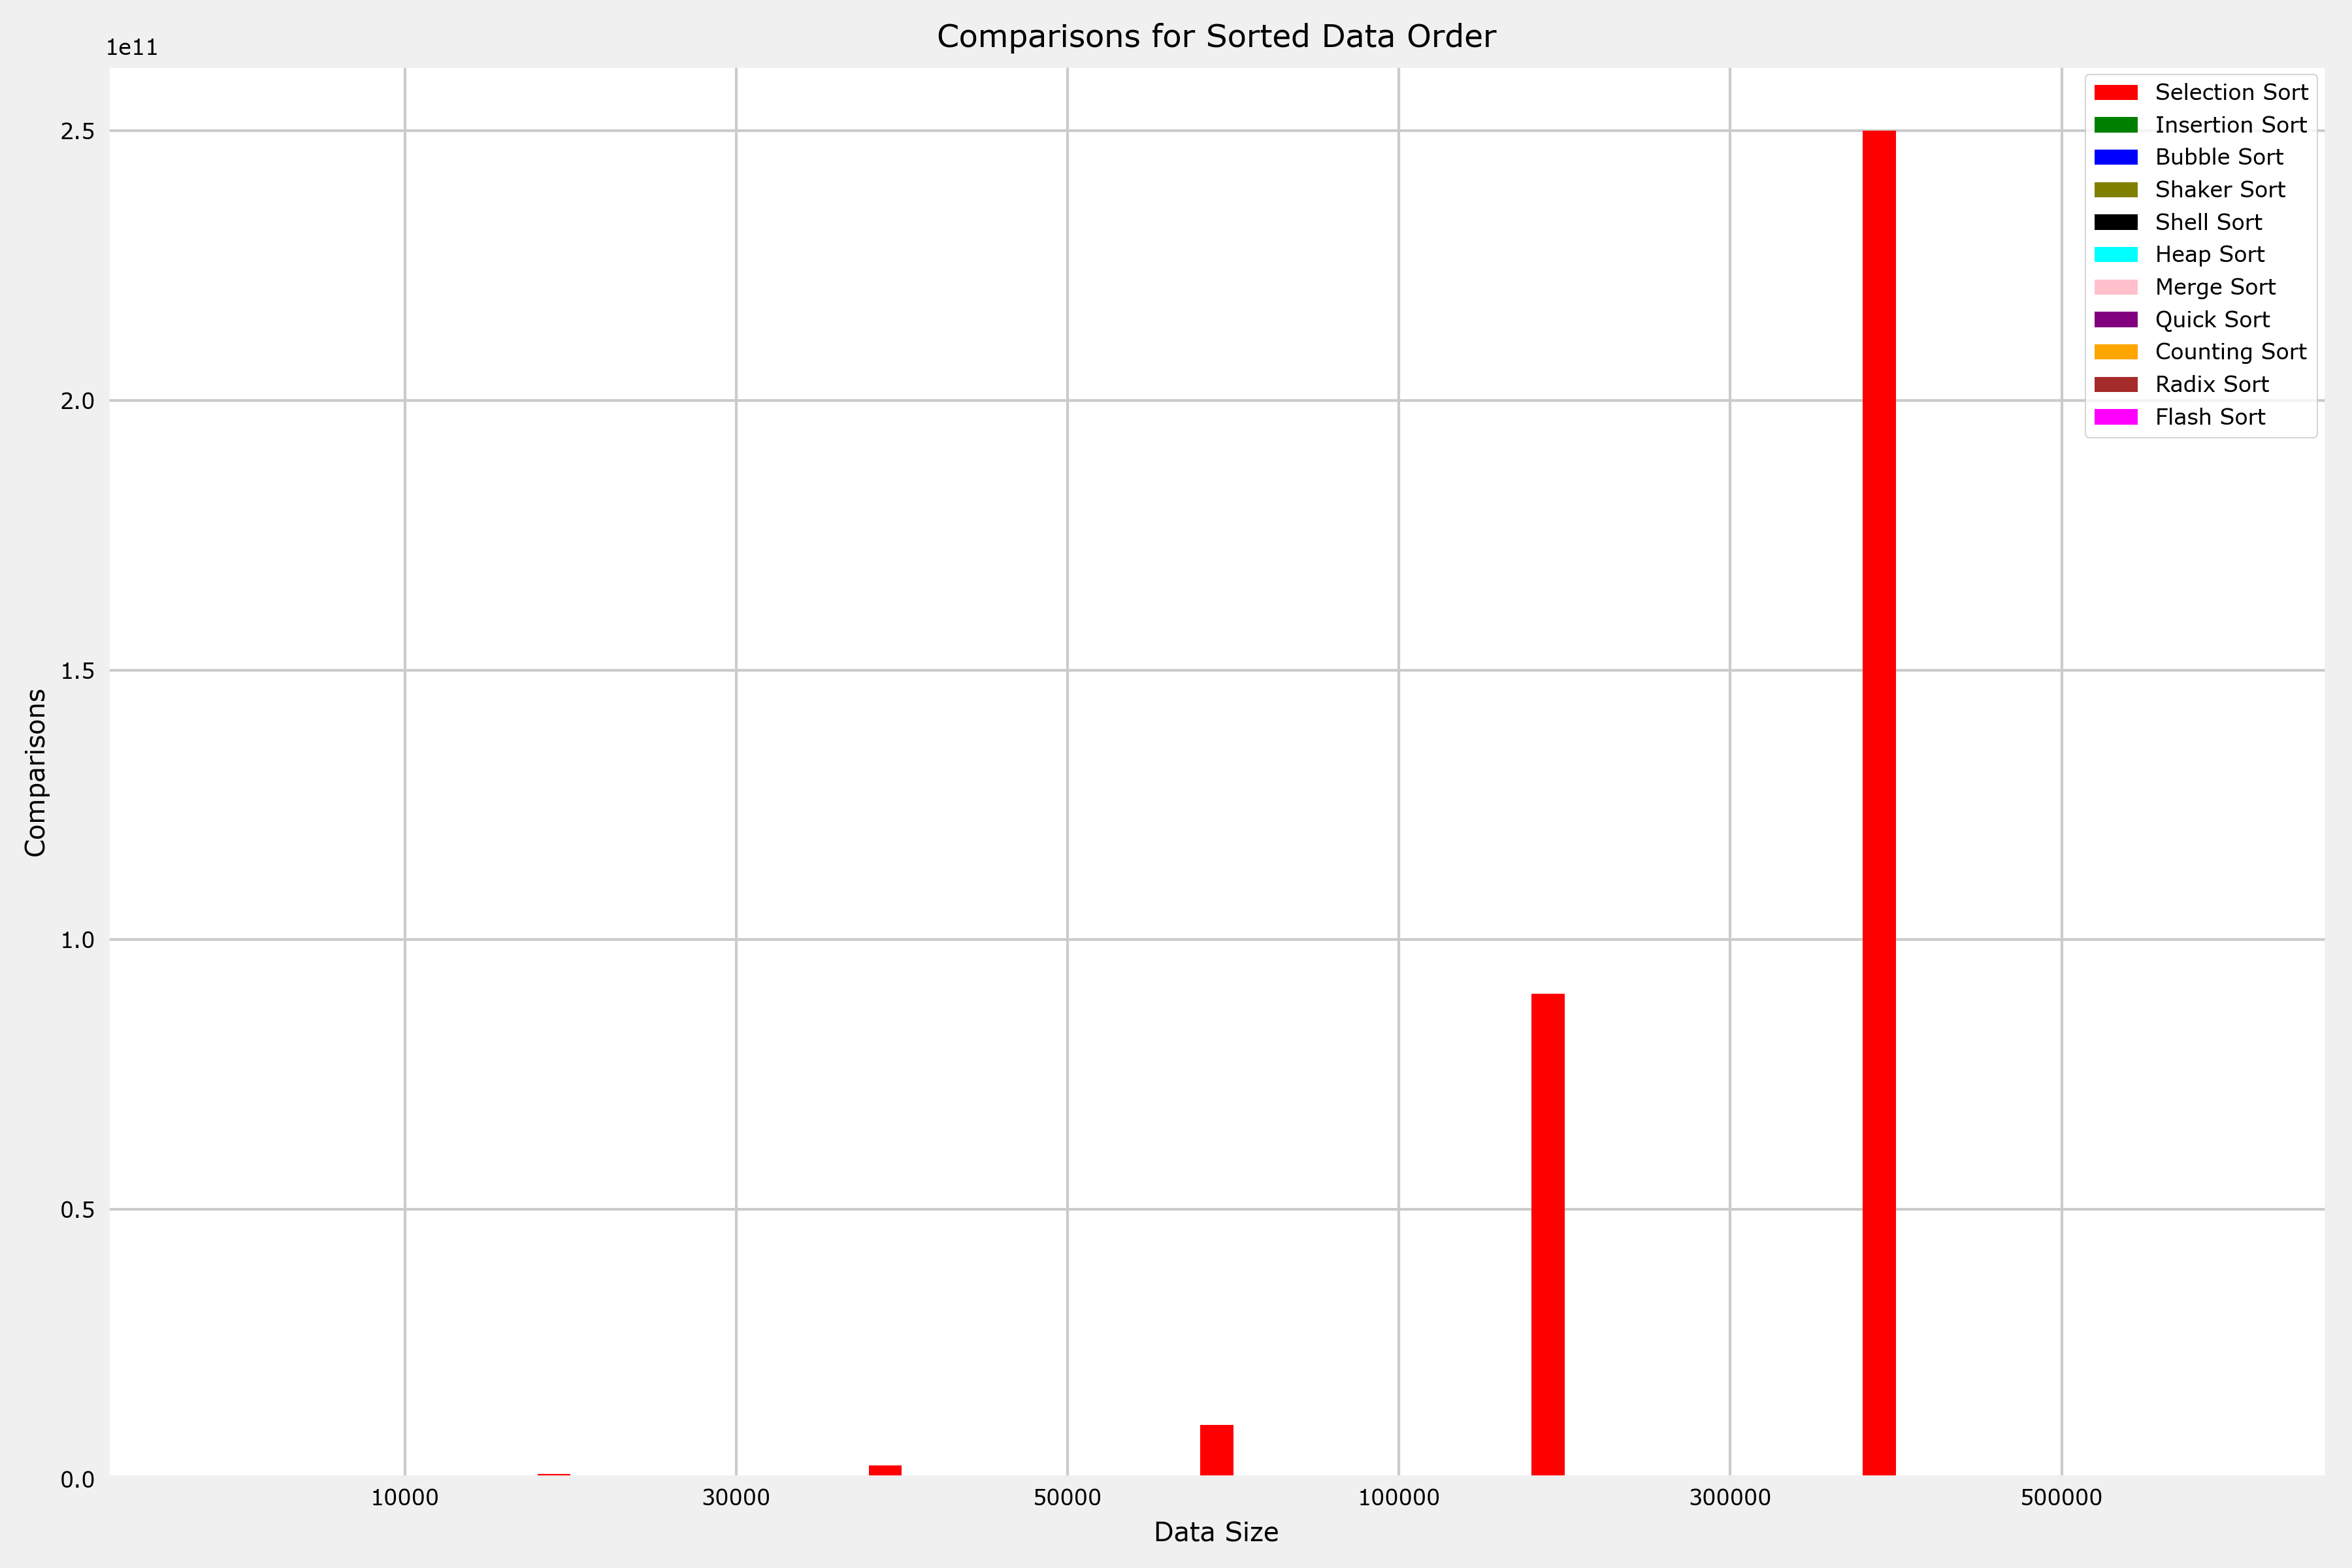
\includegraphics[width=0.8\textwidth]{img/results/sorted_comparisons.png}
    \caption{Số phép so sánh của 11 thuật toán với dữ liệu được sắp xếp}
\end{figure}

\begin{figure}[H]
    \centering
    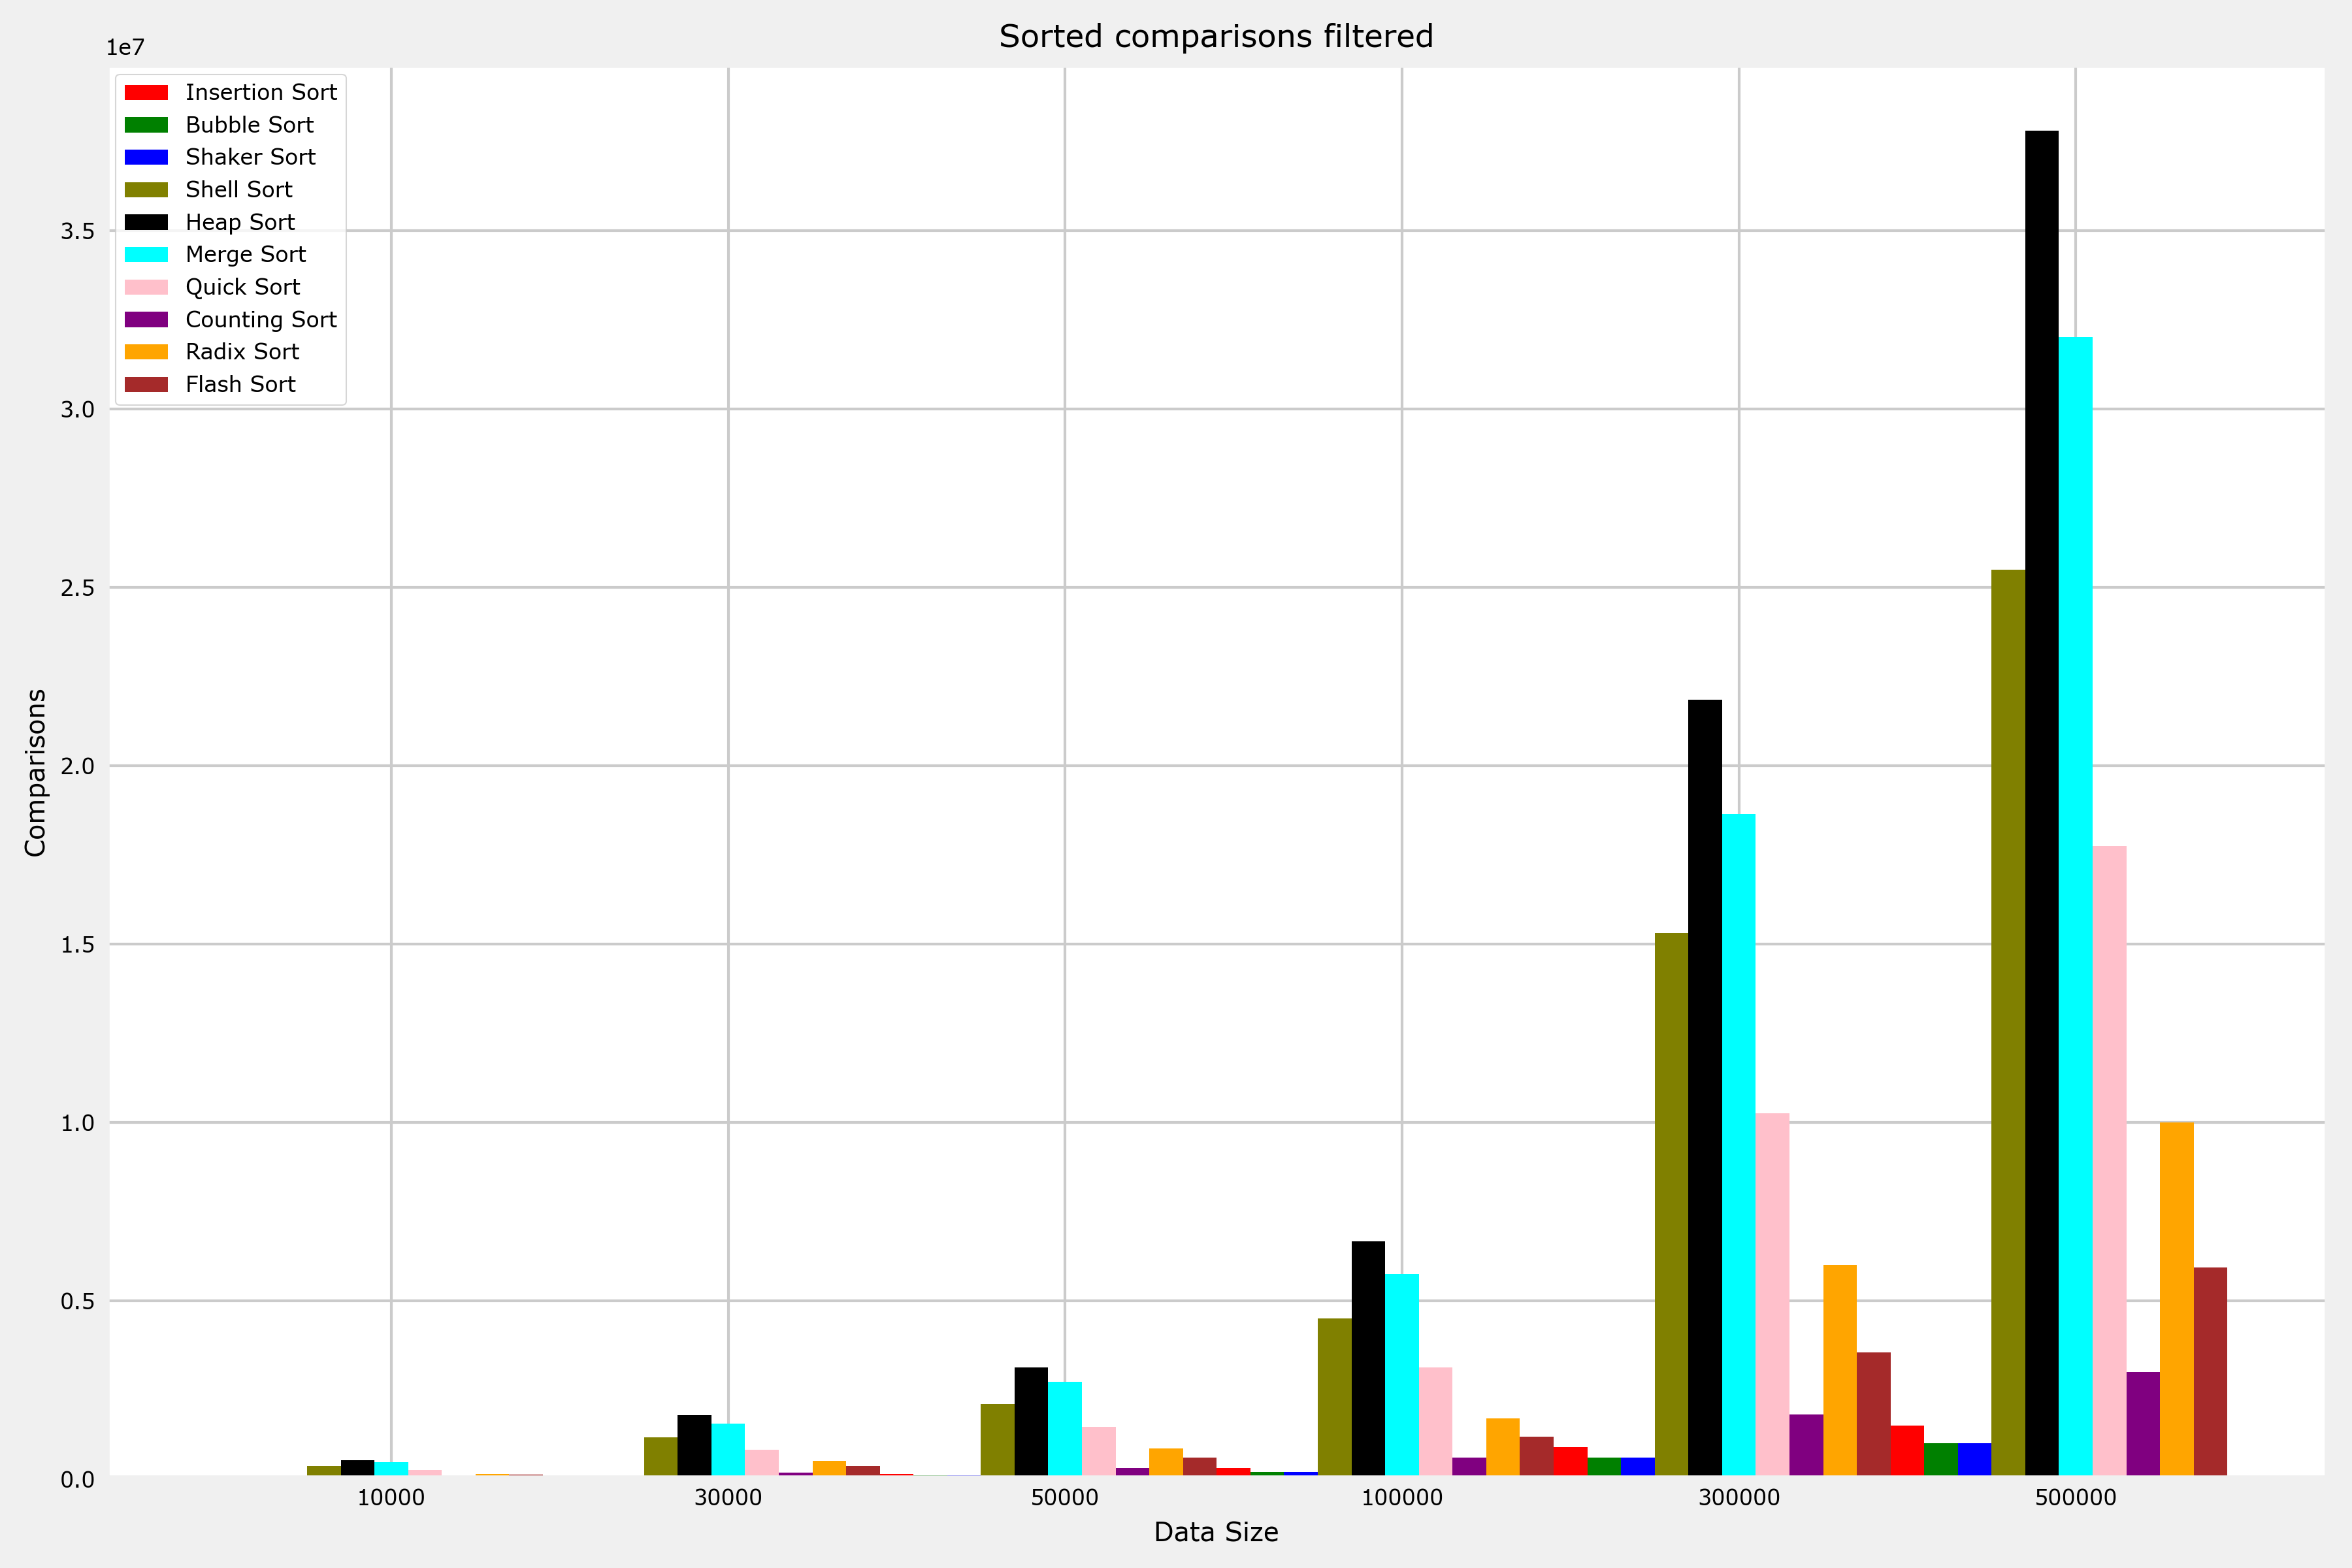
\includegraphics[width=0.8\textwidth]{img/results/sorted_comparisons_filtered.png}
    \caption{Số phép so sánh của 11 thuật toán với dữ liệu được sắp xếp sau khi loại bỏ outlier}
\end{figure}




\paragraph{4. Dữ liệu đảo ngược}
\begin{figure}[H]
    \centering
    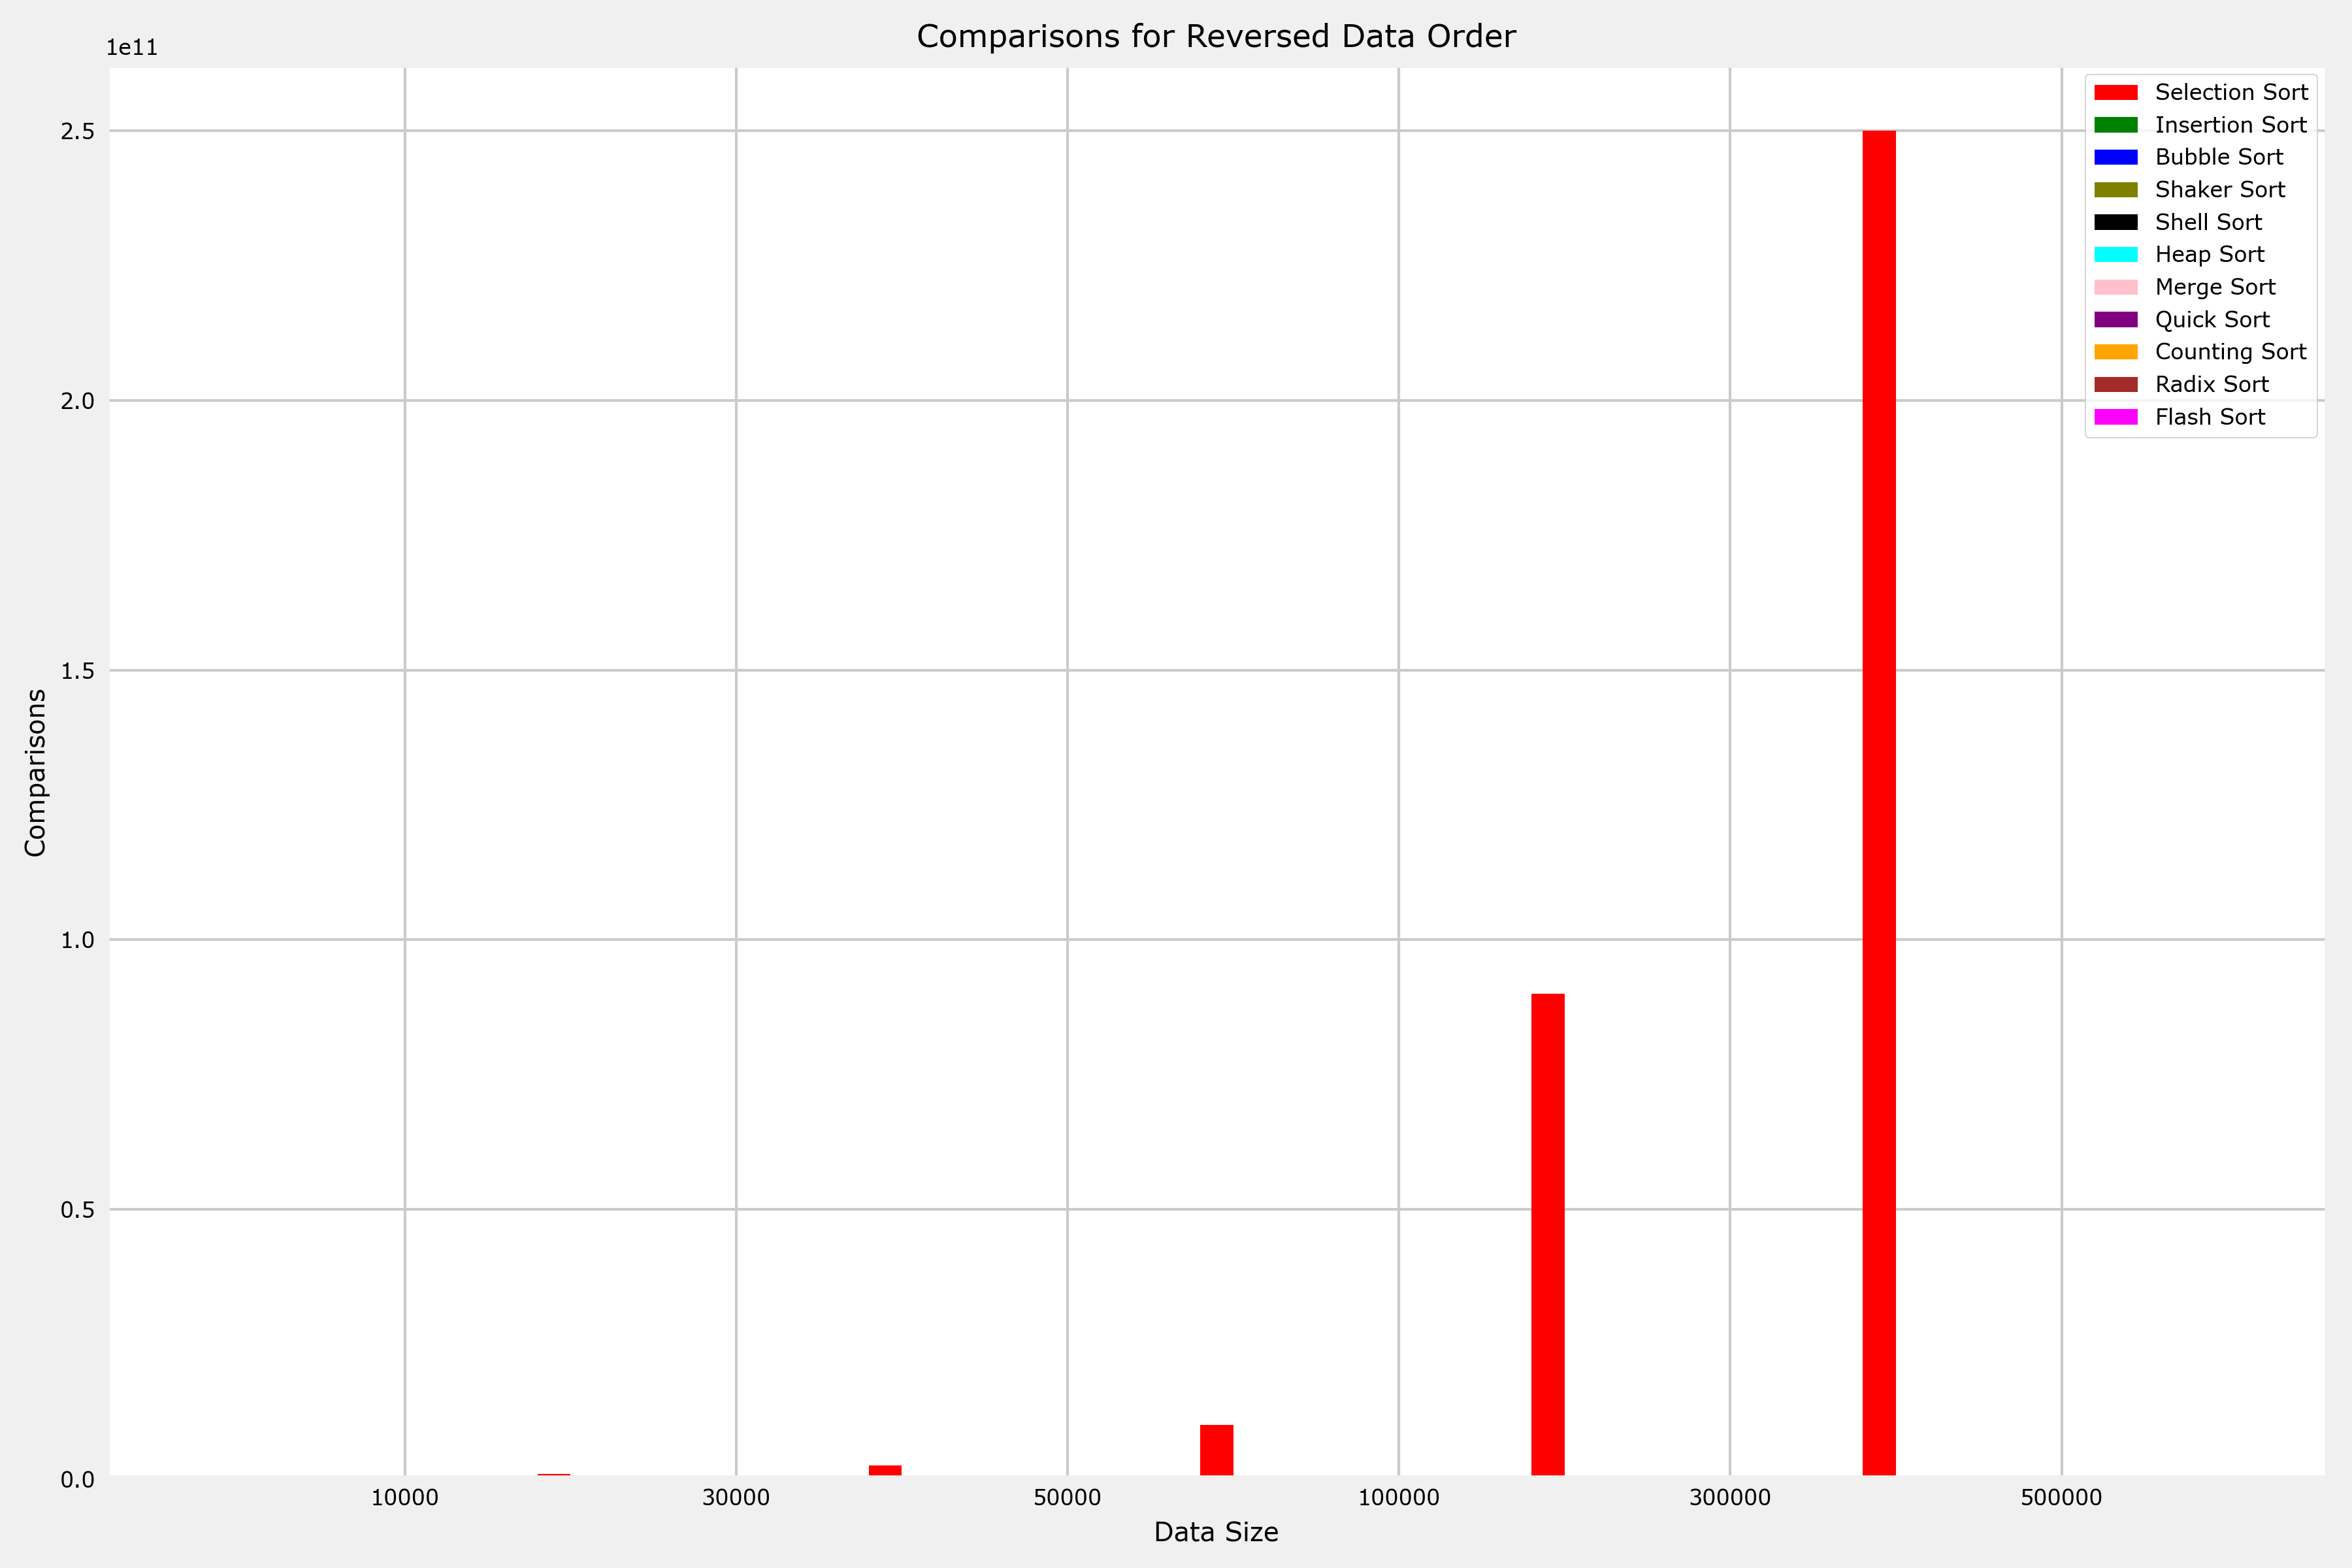
\includegraphics[width=0.8\textwidth]{img/results/reversed_comparisons.png}
    \caption{Số phép so sánh của 11 thuật toán với dữ liệu đảo ngược}
\end{figure}

\begin{figure}[H]
    \centering
    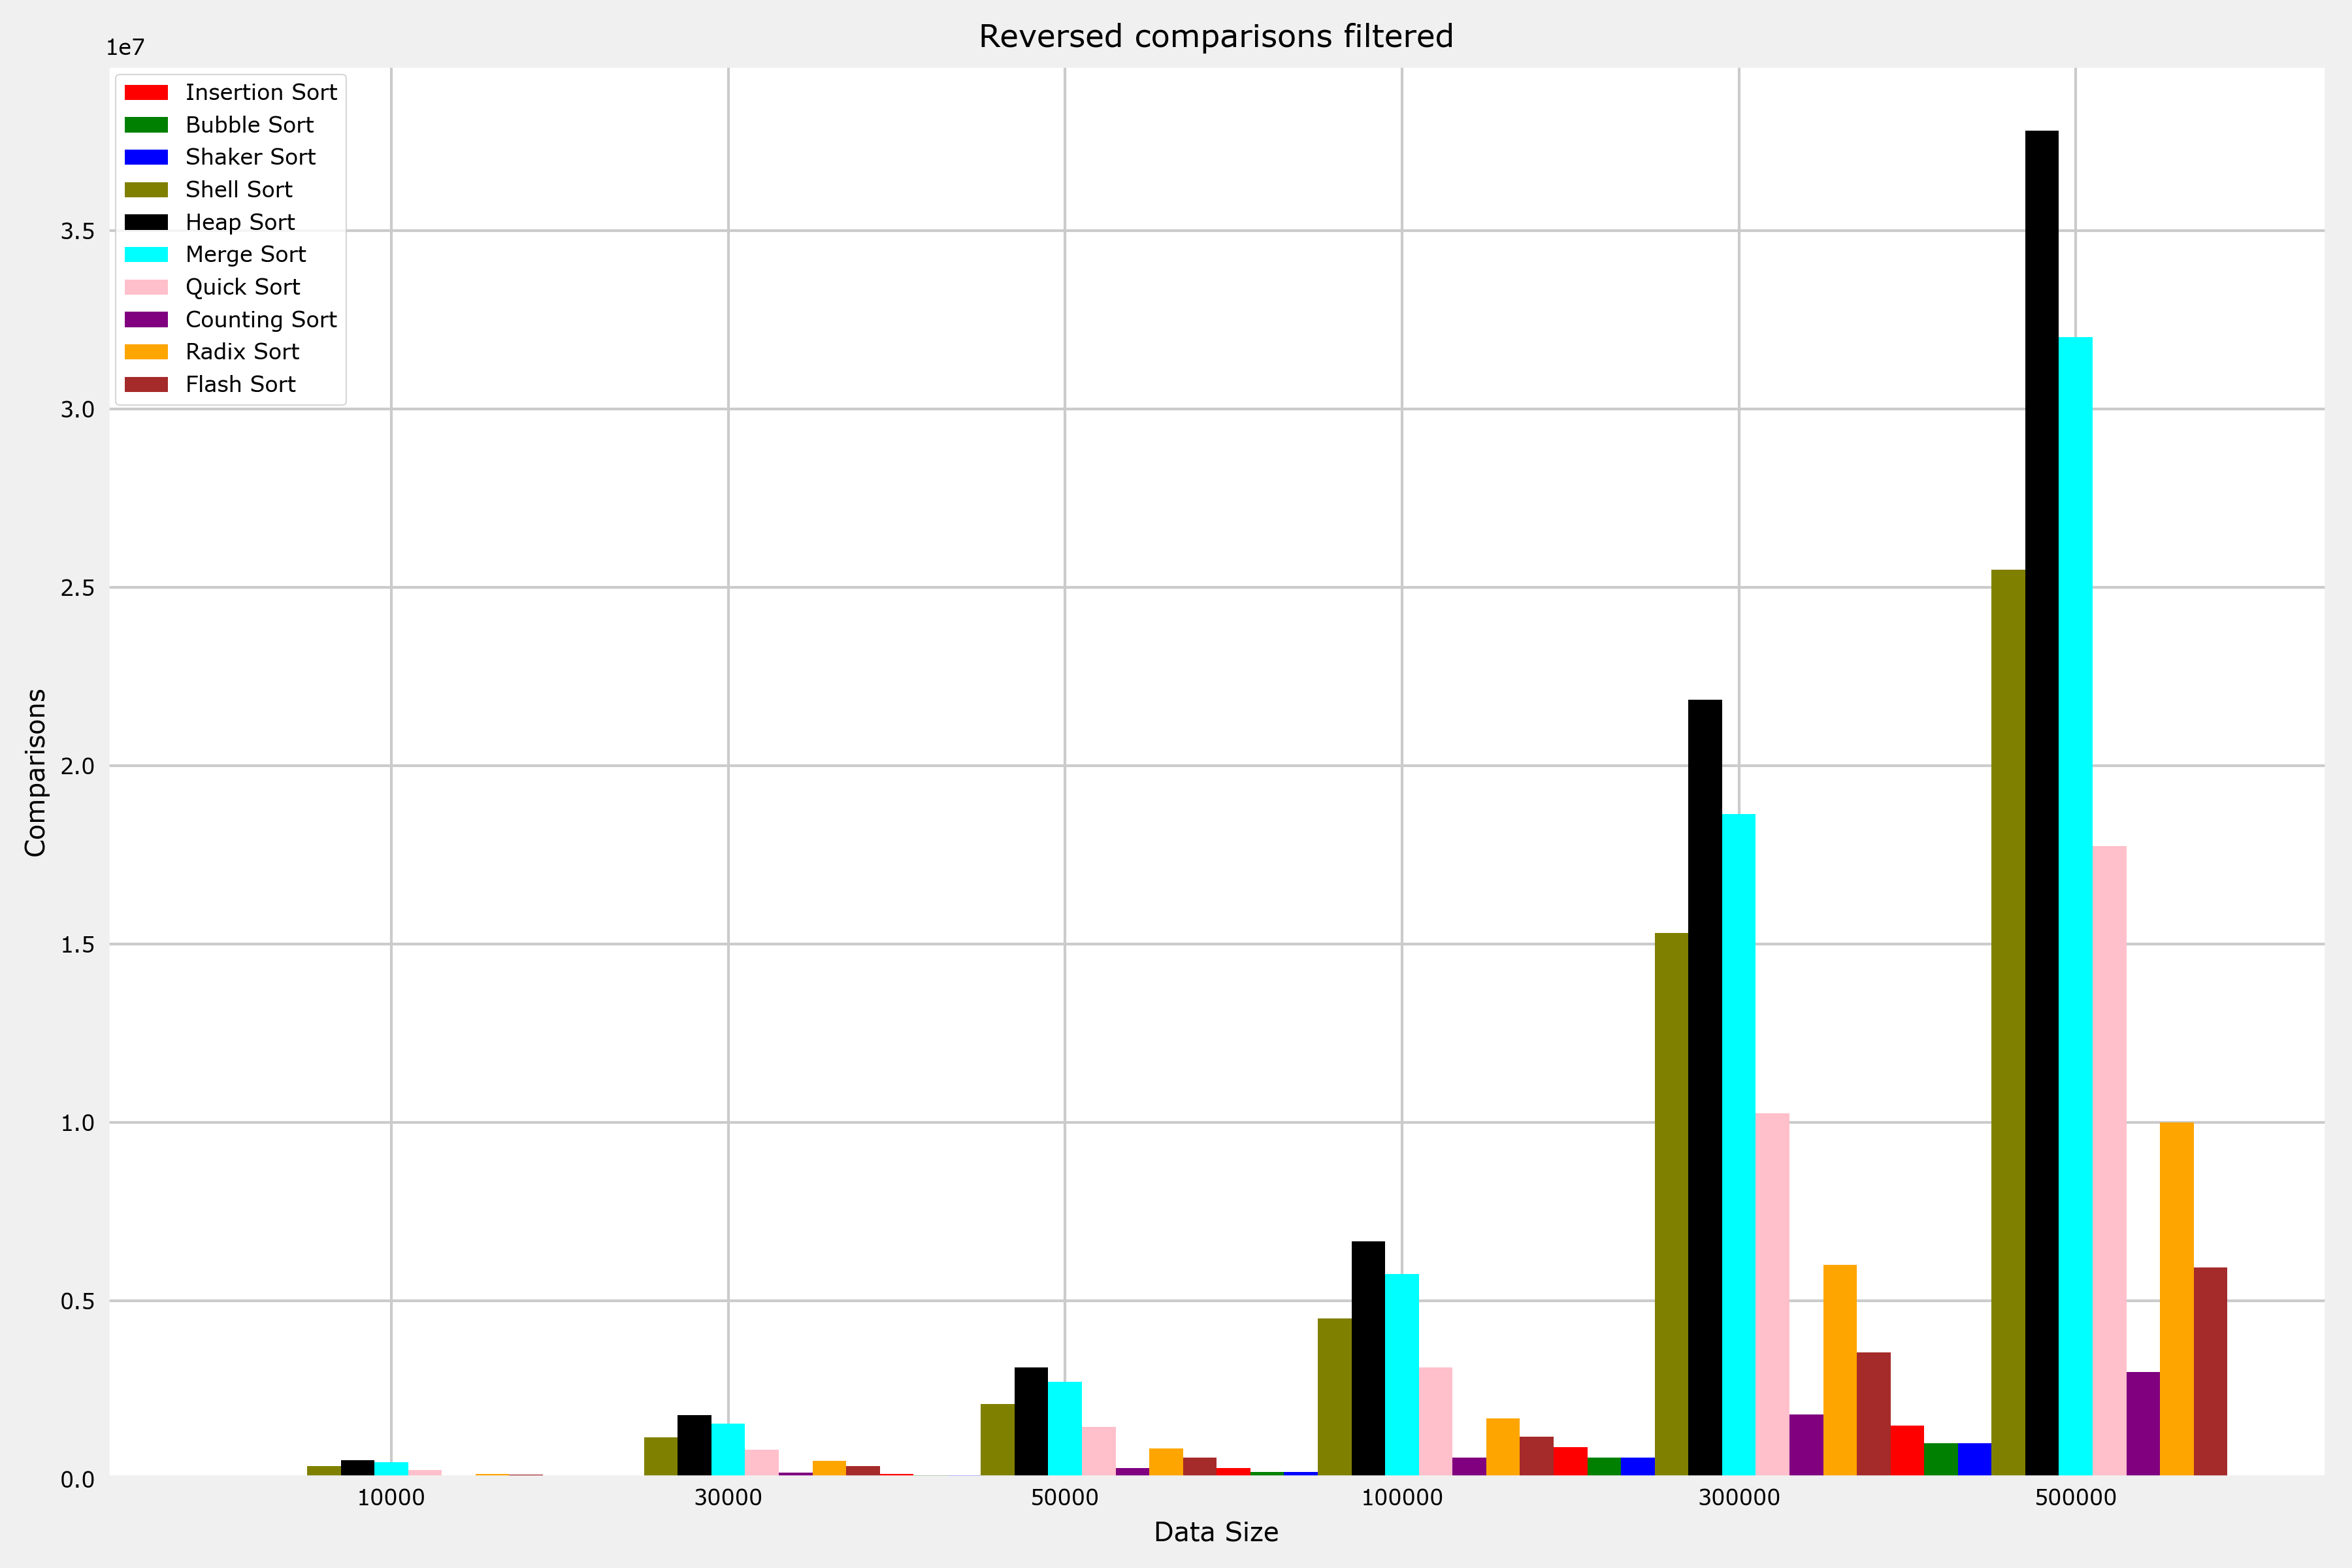
\includegraphics[width=0.8\textwidth]{img/results/reversed_comparisons_filtered.png}
    \caption{
        Số phép so sánh của 11 thuật toán với dữ liệu đảo ngược sau khi loại bỏ outlier
    }
\end{figure}